\documentclass{article}
\author{Toby {Cathcart Burn}}
\title{The Area of the Pythagoras Tree}

\usepackage{tikz}
\usetikzlibrary{automata,positioning} 
%\usetikzlibrary{lindenmayersystems}
\usepackage{ifthen}
\usepackage{pgf}
\usepackage{wrapfig}
\usepackage{amssymb}
\usepackage{amsthm}

\newtheorem*{remark}{Remark}

\newcommand{\bounding}{
\draw[tsty] (-2.5,1) -- (-1.5,0) -- (2.5,0) -- (3.5,1) -- (3.5,2.5) -- (2,4) -- (-1,4) -- (-2.5, 2.5) -- cycle;
%\draw[tsty] (-3,1) -- (-2,0) -- (3,0) -- (4,1) -- (4,2) -- (2,4) -- (-1,4) -- (-3, 2) -- cycle;
}

\newcommand{\subt}[2]{
    \begin{scope}[yshift=1cm,rotate=45,scale=0.7071]
        #1
    \end{scope}
    \begin{scope}[xshift=0.5cm,yshift=1.5cm,rotate=-45,scale=0.7071]
        #2
    \end{scope}
}
\newcommand{\dup}[1]{\subt{#1}{#1}}
\newcommand{\gtree}[3]{
	#2
	\ifthenelse{#1<2}{
		#3
	}{
		\dup{\gtree{\the\numexpr#1-1}{#2}{#3}}
	}
}
\newcommand{\tree}[1]{
	\gtree{#1}{\fill[tsty] (0,0) -- (1,0) -- (1,1) -- (0,1) -- cycle;}{}
}
\newcommand{\outertree}[1]{
	\gtree{#1}{
		\fill[tsty] (0,0) -- (1,0) -- (1,1) -- (0,1) -- cycle;
	}{\bounding}
}
\newcommand{\cdragon}[2]{
	\gtree{#1}{}{#2}
}
\newcommand{\depth}{5}%Means that rendering doesn't take so long while 
\begin{document}
\maketitle
\begin{abstract}
The area of the Pythagoras Tree is exactly
    
${12823413011547414368862997525616691741041579688920794331363953564934456759066858494476606822552437442098640979}\over{877512406035620068631903180662851572553488753575243048137500508983979170248733422547196905684808937723408093}$.
    
This can be shown by describing the Pythagoras Tree using a non-deterministic Buchi automaton with 103 states %(28-3)*4-2+1+4
and a 4 symbol alphabet.
\end{abstract}
\section{Introduction}\label{sec:intro}
The Pythagoras Tree is a fractal constructed by taking a unit square and then recursively constructing 2 copies of the Pythagoras tree each scaled by a factor of $1/\sqrt{2}$ and rotated $45^\circ$ so that the bases of the copies of the original square form a right-angled isosceles triangle with the top edge of the original square.

\begin{center}
    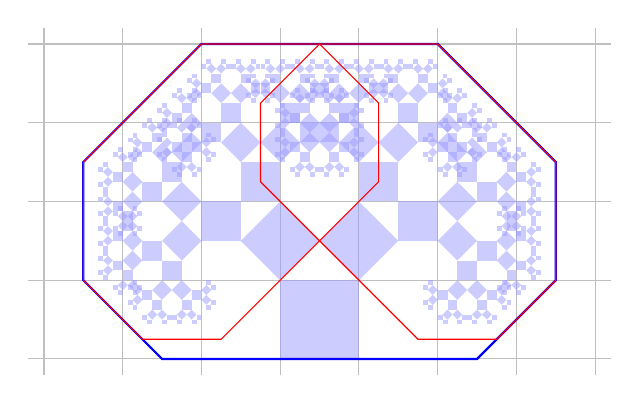
\begin{tikzpicture}[scale=1]
\draw[color=lightgray, step=1] (-3.2,-0.2) grid (4.2,4.2);
    \tikzstyle{tsty}=[fill=blue!40,opacity=0.5]
\tree{9}
\tikzstyle{tsty}=[color=blue,thick]
\bounding
\tikzstyle{tsty}=[color=red]
\dup{
    \bounding
}
\end{tikzpicture}
\end{center}
In this paper, we show that the shape can be decomposed into a finite set of squares, each of which can be split into 4 elements of the same set. This gives rise to a system of linear equations which can be solved to give an exact rational number for the area of the shape.

\newpage
\section{Defintions}
\subsection{The Pythagoras Tree}

\begin{wrapfigure}{l}{1.5cm}
	\centering
	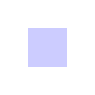
\begin{tikzpicture}[scale=0.5]
		\tikzstyle{tsty}=[fill=blue!40,opacity=0.5]
		\tree{1}
	\end{tikzpicture}
	
	Depth 1
	
	\vspace{10pt}
	
	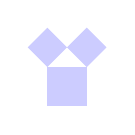
\begin{tikzpicture}[scale=0.5]
		\tikzstyle{tsty}=[fill=blue!40,opacity=0.5]
		\tree{2}
	\end{tikzpicture}
	
	Depth 2
	
	\vspace{10pt}
	
	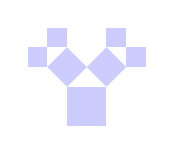
\begin{tikzpicture}[scale=0.5]
		\tikzstyle{tsty}=[fill=blue!40,opacity=0.5]
		\tree{3}
	\end{tikzpicture}
	
	Depth 3
	
\end{wrapfigure}

Let $d_0$ be the transformation which rotates 45 degrees anticlockwise and scales by $1/\sqrt{2}$ centered on $(-1,1)$
and let $d_1$ be the transformation which rotates 45 degrees clockwise and scales by $1/\sqrt{2}$ centered on $(2,1)$.

We define the \emph{depth 1 rendering} of the Pythagoras tree to consist of a unit square with opposite corners at $(0,0)$ and $(1,1)$, and the depth $n+1$ rendering to consist of 2 copies of the depth $n$ rendering transformed by $d_0$ and $d_1$ together with the unit square of the depth 1 rendering. This gives the arrangement described in Sec. \ref{sec:intro}. The Pythagoras tree is the union of the set of finite depth renderings.


This paper sets out to find the exact area of the Pythagoras tree, which we will denote $A$. $A$ is the limit of the sequence of the areas of the depth $n$ renderings.
This sequence starts $1,2,3,4,5,5 {15\over 16},6 {53\over 64},\cdots$. The limit of this monotone sequence exists since it is bounded above by the area of a $7 \times 4$ rectangle which no part of the shape leaves.

\subsection{Closure}
Whether the squares are open or closed has no effect on the area of a finite depth rendering, therefore has no effect on the limit of the sequence of areas. Since the Pythagoras tree is not closed, even if closed squares are used rather than open ones, 
Whether the closure of the limit of the sequence has a different area from the limit of the sequence is a different question that could be addressed directly, but will be shown to be false in the process of finding the area. 

\begin{remark}
	It is tempting to say (for convenience when dealing with automata) that the axis-aligned squares (added at odd depths) are closed while the other squares are open, but that smells a bit.
\end{remark}



\begin{wrapfigure}{l}{2.1cm}
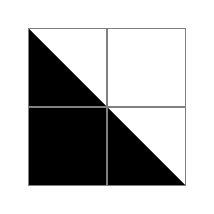
\begin{tikzpicture}
\fill (0,0) -- (2,0) -- (0,2) -- cycle;
\draw[gray] (0,0) grid (2,2);
\end{tikzpicture}
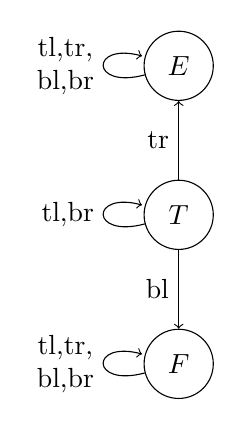
\begin{tikzpicture}[auto]
\node[state] (t) {$T$};
\node[state] (e) [above=of t] {$E$};
\node[state] (f) [below=of t] {$F$};
\path[->]
(t) edge node[swap] {bl} (f)
    edge node {tr} (e)
    edge [loop left] node {tl,br} ()
(e) edge [loop left] node[align=center] {tl,tr,\\bl,br} ()
(f) edge [loop left] node[align=center] {tl,tr,\\bl,br} ();
\end{tikzpicture}
\end{wrapfigure}

Certain subsets of a unit square can be represented by dividing the square into 4 corners and describing what each looks like. For shapes in which parts are copies of the whole, this can be done using a finite state automaton with the alphabet consisting of 4 symbols: tl (top left), tr (top right), bl (bottom left) and br (bottom right). For example, the triangle shown to the left can be described by the automaton below it. The top left and bottom right corners are smaller copies of the triangle, while the bottom left and top right corners are full and empty respectively.

This representation lets us calculate the area of the triangle. Call the area of the triangle $A_T$. Since the area of the triangle is the sum of the areas of each of the 4 corners, we have that $A_T = A_F/4 + 2A_T/4 + A_E/4$ where $A_F$ is the area of a full square and $A_E$ is the area of an empty square. As $A_F=1$ and $A_E=0$, we the equation becomes $A_T = 1/4 + A_T/2$. This lets us conclude that $A_T = 1/2$ i.e. the area of the triangle is exactly half that of the unit square.

\begin{remark}
	Technically we're using $\omega$-automata, which accept or reject infinte strings (F is the only accepting state, and every path that reaches it stays there forever, so we don't need a very fancy acceptance condition).
	Some points have multiple representations as infinite strings, but almost all of them don't, so we don't need to worry about them when calculating the area - formally, we are describing the points of the shape such that neither the x nor the y coordinate can be expressed as $a \cdotp 2^b$ where a and b are integers. The excluded subset has measure 0, so this does not affect our calculation of the area.
	
	Every open subset of the unit square can be described in this manner, if infinitely many states are allowed.
\end{remark}

\subsection{Non-deterministic Automata}
Overlapping shapes can be described by non-deterministic automata where each node may have multiple (or zero) edges with a given label. In this case we don't need a separate state for empty squares - if a corner of a node is empty, it may simply have no outgoing edges with that label.

For our purposes, any given non-deterministic automaton may be converted to a deterministic automaton by having a node in the new one for every set of nodes in the old one. The node corresponding to the set $S$ should have an edge labeled $l$ to set of all nodes in the old automaton with edges labeled $l$ from some element of $S$, and all sets containing the full node $F$ may be collapsed into one, with edges to itself.


\section{Describing the Pythagoras tree using an automaton}
One way to look at the Pythagoras tree is as 4 copies of itself, together with the 3 squares in the depth 2 rendering.
\begin{center}
	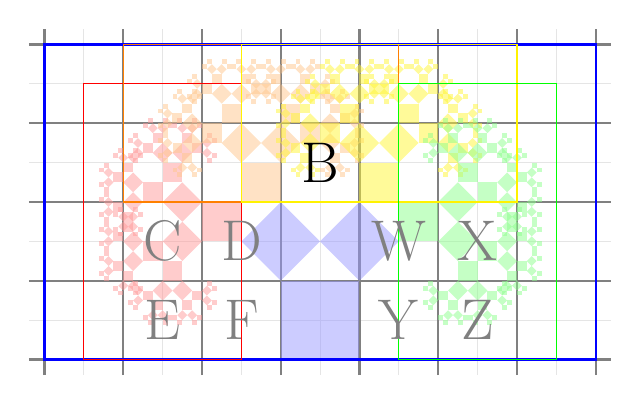
\begin{tikzpicture}[scale=1]
		\draw[color=lightgray!40, step=0.5] (-3.2,-0.2) grid (4.2,4.2);
		\draw[color=gray,thick, step=1] (-3.2,-0.2) grid (4.2,4.2);
		\draw[color=red] (-3,0) rectangle (4,4);
		\tikzstyle{tsty}=[fill=blue!40,opacity=0.5]
		\tree{2}
		\subt{\subt{
				\tikzstyle{tsty}=[fill=red!40,opacity=0.5]
				\tree{7}
			}{
				\tikzstyle{tsty}=[fill=orange!45,opacity=0.5]
				\tree{7}
		}}{\subt{
				\tikzstyle{tsty}=[fill=yellow!80,opacity=0.5]
				\tree{7}
			}{
				\tikzstyle{tsty}=[fill=green!45,opacity=0.5]
				\tree{7}
			}}
		
%		\dup{\dup{
%				\tree{7}
%		}}
		\draw[color=blue,thick] (-3,0) rectangle (4,4);
		\tikzstyle{tsty}=[color=red]
		\subt{\subt{
				\draw[color=red](-3,0) rectangle (4,4);
			}{
				\draw[color=orange](-3,0) rectangle (4,4);
		}}{\subt{
				\draw[color=yellow](-3,0) rectangle (4,4);
			}{
				\draw[color=green](-3,0) rectangle (4,4);
		}}
	\path (0.5,2.5) node[node font=\huge] {B};
	\path (-1.5,1.5) node[color=black!50,node font=\huge] {C};
	\path (-0.5,1.5) node[color=black!50,node font=\huge] {D};
	\path (-1.5,0.5) node[color=black!50,node font=\huge] {E};
	\path (-0.5,0.5) node[color=black!50,node font=\huge] {F};
	\path (1.5,1.5) node[color=black!50,node font=\huge] {W};
	\path (2.5,1.5) node[color=black!50,node font=\huge] {X};
	\path (1.5,0.5) node[color=black!50,node font=\huge] {Y};
	\path (2.5,0.5) node[color=black!50,node font=\huge] {Z};
%	\path (-1.5,0.5) node[node font=\huge] {B};
%	\dup{\dup{	\path (-1.5,0.5) node [transform shape,node font=\huge] {B};}}
%		\dup{\dup{
%			\draw[color=red] (-3,0) rectangle (4,4);
%		}}
	\end{tikzpicture}
\end{center}
The tree may be divided into 28 squares in a $7\times4$ grid so that the largest square in the tree exactly fills one square of the grid. The 4 copies described above are nicely aligned to a subdivision of the grid, allowing each square of the grid to be described as it 4 corners, each of which is either full, empty, a triangle, or an overlapping combination of squares of the original grid and their rotations. This lets us construct a non-deterministic automaton describing the shape. For example, the cell labeled B has tl-transitions to the cells C and W, tr-transitions to D and X, bl-transitions to E and Y and br-transitions to the cells F and Z. The transitions to C,D,E and F come from the yellow subtree and those labeled W,X,Y and Z come from the orange subtree.

As rotations can be multiples of $90^\circ$, we need4 states needed for each of the 28 original cells. For example, the cell labeled Y has a tr-transition to a state corresponding to Z rotated $90^\circ$ clockwise.  The transitions from rotations are straightforward given the transitions from the originals. This gives a nondeterministic automaton with $4\times28+4+1 = 117$ states (the initial 28, their rotations, 4 triangles and 1 full square). This can be transformed into a deterministic automaton with $2^{116}+1$ states, but fortunately not all of them are needed. Instead we can start from the 28 singleton sets representing squares of the grid and discover that ${\sim}10000$ states are reachable from those, which can be reduced to ${\sim}1000$ by accounting for rotations and reflections.

This gives a system of linear equations for the area of the shape described by each state. This system of equations has exactly one solution.

Noting that the area of the closure of the Pythagoras tree would also be a solution to that system of linear equations, the fact that it has a unique solution implies that taking the closure does not change the area.

\section{Details of the calculation}


\section{Further results}
We can also use this method to find the area of the Pythagoras tree with the internal triangles filled in, and to calculate the area of the Lévy C curve.

In the case of the Lévy C curve, we need a slightly different setup. Squares known to be filled don't enter the system of linear equations, so the resulting family of equations has a scaling parameter that can be maximized while ensuring that no unit square described by the automaton has an area larger than 1. This reveals that at the scale of the other diagrams, the Lévy C curve has an area of $9/4$. More conventionally, it might be scaled so that the ends are 1 unit apart, in which case the area becomes $1/4$.

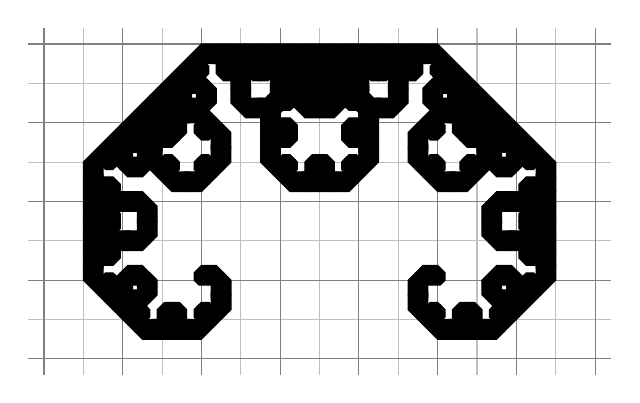
\begin{tikzpicture}[scale=1]
	\draw[color=lightgray, step=0.5] (-3.2,-0.2) grid (4.2,4.2);
	\draw[color=gray, step=1] (-3.2,-0.2) grid (4.2,4.2);
	\tikzstyle{tsty}=[fill=black]
	\gtree{9}{}{\bounding}
\end{tikzpicture}

You may question why we can take the value of an arbitrary constant to be 1 when any value between 0 and 1 would be consistent with the equations we constructed. To answer this, we need a precise definition of the Lévy C curve. Let $d_0$ be the transformation which rotates 45 degrees anticlockwise and scales by $1/\sqrt{2}$ centered on $(-1,1)$
and let $d_1$ be the transformation which rotates 45 degrees clockwise and scales by $1/\sqrt{2}$ centered on $(2,1)$. Given an infinite string $(a_i)$ in $\{0,1\}^\omega$, pick any point $p$ in $\mathbb{R}^2$, let $f(a)$ be the limit of the sequence $p,\ d_{a_1}(p),\ d_{a_1}(d_{a_2}(p)),\ d_{a_1}(d_{a_2}(d_{a_3}(p))),\ \dots$. This limit is independent of the choice of $p$. Under this definition, every point that is not outside the C dragon at some finite iteration is inside the limit. 
%    \begin{scope}[yshift=1cm,rotate=45,scale=0.7071]
%	#1
%\end{scope}
%\begin{scope}[xshift=0.5cm,yshift=1.5cm,rotate=-45,scale=0.7071]

\appendix
\section{State machine}
\section{System of Linear equations}
\section{Code}


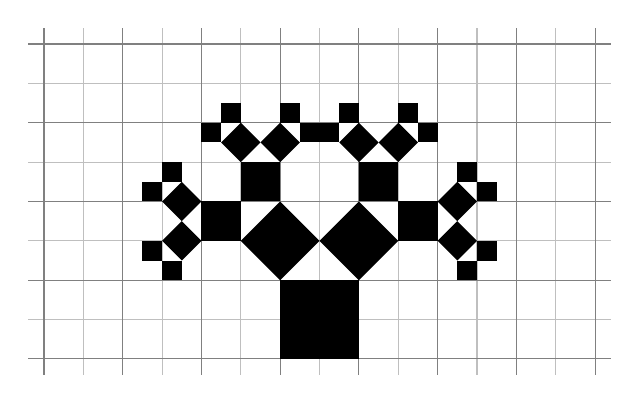
\begin{tikzpicture}[scale=1]
    \draw[color=lightgray, step=0.5] (-3.2,-0.2) grid (4.2,4.2);
    \draw[color=gray, step=1] (-3.2,-0.2) grid (4.2,4.2);
    \tikzstyle{tsty}=[]
    \tree{\depth}
\end{tikzpicture}

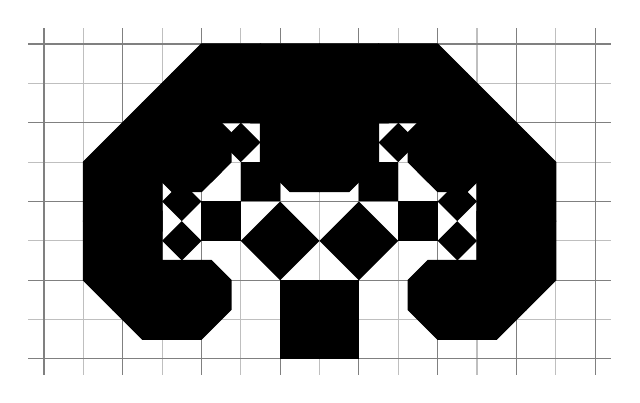
\begin{tikzpicture}[scale=1]
    \draw[color=lightgray, step=0.5] (-3.2,-0.2) grid (4.2,4.2);
    \draw[color=gray, step=1] (-3.2,-0.2) grid (4.2,4.2);
    \tikzstyle{tsty}=[fill=black]
    \outertree{\depth}
\end{tikzpicture}

\end{document}
